\subsection{The Internet}

The Internet consists of billions of connected computing devices.
End systems are also known as `hosts' and run network applications.
Computers are connected via communication links, which can be fibre optic, copper, radio or satellite.
End systems and different networks are connected to routers and packet switches that forward chunks of data known as `packets'.

The Internet is a network of networks and interconnected Internet service providers (ISPs).
The sending and receiving of messages is controlled by protocols such as TCP, IP, HTTP, Skype and 802.11.
A set of standards exists to help manage the Internet.
Proposals for standards and protocols are published as requests for comments (RFCs), which are made available to key stakeholders to be reviewed and standardised.
The Internet Engineering Taskforce (IETF) is the governing body that oversees the development of the Internet.

The Internet is also an infrastructure that provides services to applications.
These services and applications include web, VoIP, email, games, e-commerce and social networks.
It also provides a programming interface to applications.
Web hooks allow applications to connect to the Internet.

Residential, institutional and mobile access networks each have end systems connected to an edge router.
The bandwidth of a connection is affected by the hardware and connection used.
Radio links are shared, whereas an Ethernet cable is dedicated.
\begin{itemize}
  \item Network Edge:
  \newline
  Consists of the hosts/endsystems,both clients and servers.Hosts send packets of data to their access network.
  \item Access networks:
  \newline
  The physical wired/wireless communication links that connect edge systems to the core.These are the first routers that see the data packets and forward them to the network core.
  \item Network core: 
  \newline
  The central network of networks: a mesh of interconnected routers.The core routes and forwards packets of data from their source to their destination.
\end{itemize}
\begin{figure}[htp]
  \centering
  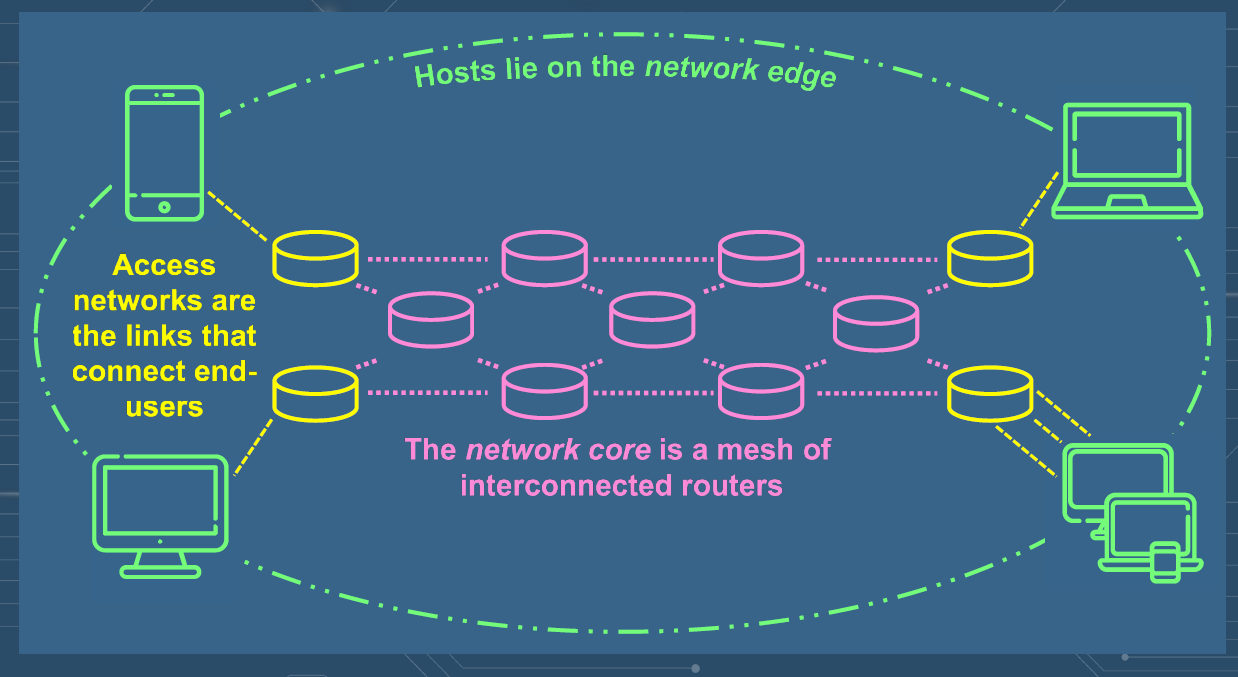
\includegraphics[width=15cm]{unit-16/figures/intro_network.png}
  \caption{Network edge/Access network/Network core}
\end{figure}
Hosts break application messages into smaller chunks known as `packets' and transmit them to the access network.
The speed at which the packet is transmitted to the access network is the link transmission rate, which is also known as `link capacity' or `link bandwidth'.
The packet transmission delay when a packet of length \( L \)~bits is transmitted into a link with transmission rate \( R \)~bits per second is \( \frac{L}{R} \)~seconds.

The network core forwards packets from one router to the next across links that form a path between source and destination.
Each packet is transmitted at full link capacity.
Routing algorithms in the network core determine the source to destination route taken by packets.
Routers forward packets from their input to their appropriate output.

\subsection{Distributed Systems}

A distributed system is one in which hardware or software components located at networked computers communicate and coordinate their actions by only passing messages.
Distributed networks allow for high concurrency.
There is no global notion of the correct time in a distributed network; there is only relative time between computers.
Each component in a network may fail independently.
The failure of one component does not affect the other components.

\subsection{Internet, Intranet and Firewalls}

The Internet is a distributed system that enables users all over the world to make use of its services.
Some highly connected links in the Internet are known as backbones.
These have high link capacity and can be connected via satellite link.

An intranet is part of the Internet that is separately administered and uses a firewall to enforce its own local security policies.
Users in an intranet share data by means of file services.

A firewall is a network security system that monitors and controls incoming and outgoing network traffic according to predetermined security rules.
A firewall establishes a barrier between a trusted internal network and an untrusted external network, such as the Internet.
Firewalls may be network-based or host-based, including network-layer or packet filters and application-layer firewalls.

\subsection{Network Principles}

Networking is concerned with sending messages over a carrier.
\begin{itemize}
  \item Latency is the term given to any kind of delay that occurs during data communication over a network.
  \item Bandwidth is the transmission capacity of a computer network or telecommunication system.
  \item Speed is the rate at which data is able to move.
\end{itemize}

A logical unit of data transmitted via a network is known as a message.
A message of arbitrary length is divided into packets before transmission.
A packet is a bit stream of restricted length.
It includes not only the data, but also relevant addressing information.

\subsection{Switching Schemes}

A network is a set of nodes connected by circuits.
In order to transmit information between two nodes, a switching scheme is required.
\begin{itemize}
  \item Broadcast --- no switching, data is transmitted throughout the network
  \item Circuit switching --- source and destination are connected through a switch at an exchange
  \item Packet switching --- a store-and-forward network with a computer at each end
\end{itemize}

\subsubsection{Circuit Switching}

End-to-end resources are allocated to create a reserved connection between source and destination.
The resources are dedicated; there is no sharing.
Full bandwidth circuit-like performance is guaranteed.
Circuit segments remain idle if not used for a connection.
This transmission scheme is traditionally used in telephone networks.

\subsubsection{Packet Switching}

Packet switching is a store-and-forward transmission scheme that allows more users to use the network.
Packets are transmitted to a router, where they are stored in a queue, waiting for an output link.
The entire packet must arrive at the router before it can be transmitted through the next link.

The delay for transmission of an \( L \)~bit packet through an \( R \)~bits per second link is \( \frac{L}{R} \)~seconds.
This is the `one-hop transmission delay'.
Assuming no propagation delay, the end-to-end delay for transmission from source to destination through one router is \( 2 \frac{L}{R} \).
In general, the delay is \( N \frac{L}{R} \), where \( N \) is the number of links and, therefore, \( N - 1 \) is the number of routers.

If the arrival rate to a router exceeds its transmission rate for a period of time, the packets will queue, waiting to be transmitted through a link.
Additionally, packets can be dropped (lost) if the memory (buffer) is filled.

\subsection{Internet Structure (Network of Networks)}

End systems connect to the Internet via access ISPs.
These may be residential, company or university ISPs.
In turn, access ISPs must be interconnected so that any two hosts can communicate.
The resulting network is very complex.
Its evolution has been driven by economics and national policies.

Connecting each access ISP to every other access ISP is not feasible.
This would require \( \function{O}{n^2} \) connections.
An alternative is to connect each access ISP to a global ISP\@.
There would be an economic agreement between customer and provider ISPs.
However, if one global ISP is a viable business, there will exist competitors, which must in turn be interconnected.

Such global ISPs are connected to each other through Internet exchange points (IXPs) or peering links.
Regional networks also exist to connect groups of access networks to global ISPs.
Large Internet companies, such as Google and Microsoft, run their own content delivery networks to bypass connections and provide services and content closer to end systems.

The result is small number of well-connected large networks.
These are `Tier~1' commercial ISPs that offer national and international coverage, and private content delivery networks that connect data centres to the Internet to bypass Tier~1 and regional ISPs.

\subsection{Packet Loss and Delays}

When the arrival rate of packets at a router exceeds the output link capacity, the packets wait in a buffer queue for transmission.
A packet is dropped (lost) if there is no available buffer space in the queue when it arrives.
A lost packet may be retransmitted by the previous node, the end system source or not at all.
Nodal delay \( d_{\text{nodal}} \) is the delay of packets at a node in a network.

\begin{equation*}
  d_{\text{nodal}} = d_{\text{proc}} + d_{\text{queue}} + d_{\text{trans}} + d_{\text{prop}}
\end{equation*}

\begin{itemize}
  \item Nodal processing delay (\( d_{\text{proc}} \))
  \begin{itemize}
    \item Time spent checking bit errors and determining output link
    \item Typically less than a millisecond
  \end{itemize}
  \item Queueing delay (\( d_{\text{queue}} \))
  \begin{itemize}
    \item Time spent waiting at output link for transmission
    \item Dependent upon congestion level at link/router
  \end{itemize}
  \item Transmission delay (\( d_{\text{trans}} \))
  \begin{itemize}
    \item Time spent placing packet onto output link
    \item For a packet of length \(L\)~\si{\bit} and link of bandwidth \(R\)~\si{\bit\per\second}, \( d_{\text{trans}} = \frac{L}{R} \)~\si{\second}
  \end{itemize}
  \item Propagation delay (\( d_{\text{prop}} \))
  \begin{itemize}
    \item Time spent travelling through output link to next node
    \item For a link of length \(d\)~\si{\metre} and a propagation speed through the link medium of \(s\)~\si{\metre\per\second}, \( d_{\text{prop}} = \frac{d}{s} \)~\si{\second}
  \end{itemize}
\end{itemize}

Throughput is the rate at which bits are transferred between sender and receiver.
Throughput can be measured as instantaneous throughput at a specific point in time or average throughput over a longer period of time.
The average end-to-end throughput is determined by the link with the lowest capacity.
A link on an end-to-end path that constrains the throughput is known as a `bottleneck link'.

\subsection{Protocols}

Network protocols define a set of guidelines that allow network devices to communicate effectively.
A protocol defines the sequence of messages that should be exchanged and the format of the data in the messages.
Protocols are implemented by pairs of software modules in the sending and receiving systems.

A transport protocol transmits a message from a sender to a receiver.
A process that wishes to send a message passes it to the transport protocol module.
The software divides the message into packets, which are then transmitted using the network protocol.
Inverse operations are performed by the receiver to reconstruct the message.

\begin{figure}[htp]
  \centering
  \includegraphics[width=15cm]{unit-16/figures/frame-part-1.png}
  \includegraphics[width=15cm]{unit-16/figures/frame-part-2.png}
  \caption*{The structure of a packet frame.}
\end{figure}

\subsection{Protocol Layers and Encapsulation}

Network software is arranged in a hierarchy of layers, in which each layer presents an interface to the layer above.
Each layer accepts an item of data in a specified format from the layer above.
It applies a transformation to the data in order to encapsulate it.
The data is passed to the layer below.
Layers communicate with those directly above and below through procedure calls.
Every computer in a network must have these layers.

A complete set of protocol layers is known as a `protocol suite' or `protocol stack'.
Each layer adds a header to the data before it is sent.

\subsection{Open Systems Interconnection (OSI) Model}

The Open Systems Interconnection (OSI) model is a conceptual protocol stack model.
Its layers from highest to lowest are
\begin{itemize}
  \item application,
  \item presentation,
  \item session,
  \item transport,
  \item network,
  \item (data) link, and
  \item physical.
\end{itemize}

Data are passed down through the layers in the source end system and across the network via physical connections.
Switches and routers use the data link and network layers to route the data through the network.
When the data arrive at the end system, they are passed up through the layers and are reconstructed.

\begin{table}[htp]
  \centering
  \caption*{The layers of the OSI model.}
  \includegraphics[width=15cm]{unit-16/figures/layer-summary.png}
\end{table}

Protocol layering simplifies and generalises the software interfaces that access communication services.
However, they reduce the performance of the network.
A total of \(N\) protocol layers results in \(N\) control transfers for each message at an end system, and \(N\) copies of the data due to encapsulation.
Thus, the data transfer rate may be much slower than the available network bandwidth.

The five-layer protocol stack used by the Internet differs from the seven-layer OSI model.
Its layers from highest to lowest are
\begin{itemize}
  \item application,
  \item transport,
  \item network,
  \item link, and
  \item physical.
\end{itemize}
The application, presentation and session layers of the OSI model are not clearly distinguished in the Internet protocol stack, and are instead all part of a single application layer.
Applications are responsible for deciding how to handle these protocols.
The session layer is integrated with the transport layer.

{\color{red} \textbf{The contents in grey are not included in syllabus any more.}}

{\color{gray}
\subsection{Large Messages and Message Consistency}
An Ethernet frame can only hold \SI{1500}{\byte} of data.
Messages larger than this limit must be broken into packets.
Message consistency and reliable data transfer are achieved by communicating via the Transmission Control Protocol (TCP).
If there are errors in the packets, the receiver notifies the sender, and those packets are sent again.
If the message is a single long packet, there may be issues due to poor connection.

Packets may not be received in the same order that they are sent.
Each packet contains a sequence number so that they can be reordered correctly.

\subsection{Ports and Addressing}
The responsibility of the transport layer is to provide a network-independent message transfer service between pairs of network ports.
The destination ports at a host computer are defined by software and are attached to processes.
Port~\num{25} is used for email.

The transport layer delivers messages to destinations specified by transport addresses.
A transport address comprises a network address and a port number.
In the Internet, every host system is assigned an Internet Protocol (IP) address that identifies it and the subnet to which it is connected.

\subsection{Datagram Packet Delivery}
In datagram packet delivery, it is the responsibility of the receiver to indicate if there is a problem with transmission.
The network retains no information after it has been delivered.
The sequence of packets may take different routes from host to destination, so they may arrive out of sequence.
Datagrams contain the full network addresses of the source and destination.
The network layer of the Internet uses datagram delivery.

A link-layer switch accesses the data link layer of a packet to determine the next link to which the packet must be sent.
A router is a three-layer switch.
It accesses the network layer of the packet in order to route the packet to the destination host.
}